% Created 2020-05-24 Sun 20:01
% Intended LaTeX compiler: pdflatex
\documentclass[11pt]{article}
\usepackage[utf8]{inputenc}
\usepackage[T1]{fontenc}
\usepackage{graphicx}
\usepackage{grffile}
\usepackage{longtable}
\usepackage{wrapfig}
\usepackage{rotating}
\usepackage[normalem]{ulem}
\usepackage{amsmath}
\usepackage{textcomp}
\usepackage{amssymb}
\usepackage{capt-of}
\usepackage{hyperref}
\usepackage{minted}
\author{Dustin Leatherman}
\date{\today}
\title{Class Notes}
\hypersetup{
 pdfauthor={Dustin Leatherman},
 pdftitle={Class Notes},
 pdfkeywords={},
 pdfsubject={},
 pdfcreator={Emacs 26.3 (Org mode 9.4)}, 
 pdflang={English}}
\begin{document}

\maketitle
\tableofcontents


\section{Review \& Introduction (2020/04/02)}
\label{sec:orgf218f8e}

\textbf{Monte Carlo Simulations}: A family of computational algorithms using repeated
 sampling to get numerical results.


\textbf{Applications}
\begin{itemize}
\item get deterministic results
\item Approximate High Dimension Integration
\end{itemize}

\subsection{Review}
\label{sec:org312cd6b}

Note that since every class has a review period for the first lecture, the notes
documented here represent points that were either stressed or that I found
particularly interesting
\subsubsection{Distributions by Question}
\label{sec:org2c62abf}

\textbf{Binomial}
\begin{itemize}
\item How \emph{many} basketball free throws do you make out of a given number of attempts?
\item How \emph{many} people prefer the iPhone to other smart phones?
\end{itemize}

\textbf{Poisson}
\begin{itemize}
\item How \emph{many} taxis pass by your corner in a given time?
\item How \emph{many} servers crash in a given time?
\end{itemize}

\textbf{Gamma Distribution}
\begin{itemize}
\item How \emph{long} does it take for the next \emph{several} taxis to pass by your corner?
\item How \emph{long} does it take for the next \emph{several} servers to crash in a given time?
\end{itemize}

\textbf{Gaussian}
\begin{itemize}
\item How \emph{far} does a stock price move in a given period of time?
\item Describe averages
\end{itemize}

\begin{enumerate}
\item Gamma
\label{sec:org9c310d5}

Time it takes for the next several taxis to pass by.

\(T ~ Gamma(\alpha, \beta)\)

\(\beta\): Average waiting between taxis

\(\alpha\): number of taxis

\begin{quote}
I noted this because I haven't used the Gamma distribution too much and I
thought this was an intuitive way to describe it.
\end{quote}
\end{enumerate}

\subsubsection{Independence}
\label{sec:orgf0b4437}

If \(Y_1 \sim N, Y_2 \sim N\), they are Bivariate Normal

If \(\sigma_{12} = 0\), \(Y_1, Y_2\) are independent since \(\sigma_{12} = cov(Y_1,
Y_2) = 0\).

\begin{enumerate}
\item Proof
\label{sec:orge58e342}

Any Bivariate Normal Random Var can be written as a linear function of two
independent Normal R.V.s.

\begin{equation}
\begin{split}
x_1 = & z_1\\
x_2 = & \sigma_{12} z_1 \pm z_2 \sqrt{1 - \sigma_{12}^2}
\end{split}
\end{equation}


\begin{equation}
\begin{split}
cov(x_1, x_2) = \ & cov(z_1, \sigma_{12} z_1 \pm z_2 \sqrt{1 - \sigma_{12}^2})\\
= \ & cov(z_1, \sigma_{12} z_1 \pm z_2 \sqrt{1 - \sigma_{12}^2})\\
= \ & cov(z_1, \sigma_{12} z_1) + cov(z_1, z_2 \sqrt{1 - \sigma_{12}^2})\\
= \ & \sigma_{12} V(z_1) + 0\\
= \ & \sigma_{12}
\end{split}
\end{equation}

if \(\sigma_{12} \new 0\), x,y are \textbf{not} independent

if \(\sigma_{12} = 0\),
\begin{itemize}
\item \(x_1 = z_1\)
\item \(x_2 = z_2\)
\end{itemize}

This implies that \(x_1\) and \(x_2\) are independent.
\end{enumerate}

\subsection{Introduction}
\label{sec:orgce8814d}

\begin{quote}
Metropolis Sampling - important method in Bayesian Statistics
\end{quote}

Y represents some interesting quantity
\begin{itemize}
\item result of a game
\item payoff of a derivative option
\item daily profit
\item time taken to travel by car to work
\end{itemize}

Compute the mean, \(E(Y) = \mu\)
\begin{itemize}
\item probability of winning
\item fair price of a derivative option purchased today
\item average daily profit
\end{itemize}

Or Y can be a percentile

The idea is to generate samples of Y with the \emph{same} distribution to compute the
sample mean, percentile as estimates of the true quantities.

\subsection{Big Questions}
\label{sec:orga4360df}

\begin{itemize}
\item How do we generate the \(Y_i\) with a complicated distribution? Often \(Y_i =
  f(X)\), where \(X = (X_{i1}, ..., X_{id})\) is easy to generate and \(f\) is known.
\item How do we generate \(X_i\) above?
\item How large does \emph{n} need to be?
\item Can we reduce n(time, cost) by being clever?
Yes, by choosing \(Y_i\) more carefully?
\end{itemize}

if \(cov(Y_i, Y_j) = \rho\):

\begin{equation}
\begin{split}
V(\bar{Y}) = & \frac{\sigma^2}{n} + \frac{2n(n - 1)}{n^2} cov(Y_i, Y_j)\\
= & \frac{\sigma^2}{n} + \frac{n(n - 1)}{n^2} \rho \sigma^2
\end{split}
\end{equation}

\subsection{Example: Interest Rate}
\label{sec:orgafb5282}

k = number of times per year interest is compounded
\(r_k\) = interest rate per year compounded k times per year
\(r_1\) = annualized percentage rate (APR)
\(r\) = interest rate per year compounded continuously

\begin{equation}
\begin{split}
r_1 = & (1 + \frac{r_k}{k})^k - 1 = e^r - 1\\
r = & k ln(1 + \frac{r_k}{k}) = ln(1 + r_1)
\end{split}
\end{equation}

\begin{equation}
\begin{split}
    \underset{n \to \infty}{lim} (1 + \frac{1}{n})^n = & e\\
    \underset{n \to \infty}{lim} (1 + \frac{0.05}{n})^n = & \underset{n \to \infty}{lim} (1 + \frac{0.05}{n})^{\frac{n}{0.05}} = e^{0.05}
\end{split}
\end{equation}

\subsection{Example: Estimating Pi}
\label{sec:orgd2888ed}

Assume the following:
\begin{itemize}
\item a piece of 1 x 1 square wood with a circle in it
\item infinite darts
\end{itemize}


How to estimate the value of \(\pi\)?

Area of square: 1
\(r = 0.5\)
Area of a circle: \(\pi r^2 = \frac{\pi}{4}\)

\(\hat \pi = 4 \times \frac{\text{\# of darts in circle}}{\text{\# of darts in square}}\)

\subsection{Example: Sandwich Shop Profit}
\label{sec:org220d3f0}

\(D_{ij} \sim U(5, ..., 35), i = 1,...,n, j = 1,...,d\)

j: day
i: random variable

profit: \(P_{ij} = min(D_{ij}, O) R - OW\)

average daily profit over d days: \(\bar{P_i} = \frac{1}{d}(P_{i1} + ... + P_{id}), i = 1, ..., n\)

\begin{equation}
\begin{split}
\hat \mu = & \frac{1}{n}(\bar{P_1} + ... + \bar{P_n}) = \frac{1}{nd} \sum_{i,j = 1}^{n, d} P_{ij}\\
\hat \sigma^2 = & \frac{1}{n - 1} \sum_{i = 1}^{n} (\bar{P_i} - \hat \mu)^2\\
\hat \mu \pm & 2.58 \frac{\hat \sigma}{\sqrt{n}}
\end{split}
\end{equation}

2.58 is p = 0.005 for a 99\% C.I.

\subsubsection{Questions}
\label{sec:orgc5e99a4}
\begin{itemize}
\item What size order gives the maximum average daily profit? Why? Have you tried
other order sizes?
\item How accurately can you know the average daily profit from the simulation? How
does this depend on the number of days for your simulation?
\item How does the answer vary as you change your model assumptions?
\item Plot daily profit and average daily profit with the number of days
\end{itemize}
\section{Review \& Estimating Integrals (2020/04/09)}
\label{sec:org34ebb15}
\subsection{Review}
\label{sec:org3bdbeae}

\(MSE(\hat \mu) = Var(\hat \mu) + [bias(\hat \mu)]^2\)

\(bias(\hat \mu) = E(\hat \mu) - \mu\)

\textbf{Simple Monte Carlo Simulator}: \(\hat \mu = \bar Y = \frac{1}{n} (\Sigma Y_i)\)

\subsubsection{Chebyshev Inequality}
\label{sec:org6fc995e}

When working with an unknown distribute, the Chebyshev inequality can
be used to construct Confidence Intervals (albeit wide).

$$
P(|Y - \mu| < k \sigma) \geq 1 - \frac{1}{k^2}
$$

$$
P(|Y - \mu| > k \sigma) \leq \frac{1}{k^2}
$$

\subsubsection{Determining N}
\label{sec:org80a6377}

\begin{equation}
\begin{split}
|\frac{Z_{1 - \alpha/2} \hat \sigma}{\sqrt{n}}| \leq \epsilon \to n \geq (\frac{Z_{1 - \alpha/2}\hat \sigma}{\alpha})^2
\end{split}
\end{equation}

\(\hat \sigma\): Unbiased estimate of \(\sigma\)

\(\alpha\): Error tolerance.

In this class so far, \(\alpha = 0.01\)

\begin{enumerate}
\item Steps
\label{sec:org131e454}

\begin{enumerate}
\item Choose a small sample size (\(n_0 = 1000\)). Then generate \(n_0\) random samples
from an underlying probability distribution
\item Calculate \(\hat \sigma\)
\item Calculate \(n\)
\item Generate another sample of size \(n\) from the underlying probability
distribution.
\item Compute \(\hat \mu\) with error \(\pm Z_{1 - \alpha/2} \frac{\hat \sigma_n}{\sqrt{n}}\)
\end{enumerate}
\end{enumerate}

\subsection{Estimating Integrals}
\label{sec:org943f12e}

$$
\mu = \int_{R^d} g(x)dx = ?
$$

Let \(f(x) = \frac{g(x)}{\rho(x)}\) where \(\rho(x)\) is a probability density
function (PDF) and \(g(x)\) is the function of interest to be estimated.

Then,
$$
\mu = \int_{R^d} f(x) \rho(x) dx = E(Y)
$$

where \(Y = f(X)\)

\subsubsection{Example - Normal Probability}
\label{sec:orgb757e87}

$$
\mu = \int_0^1 \frac{1}{\sqrt{2 \pi}} exp(\frac{-x^2}{2}) dx = \Phi(1) - \Phi(0)
$$

$$
RMSE(\hat \mu) = \sqrt{Var(\hat \mu) + [bias(\hat \mu)]^2}
$$

Summary
\begin{center}
\begin{tabular}{lrll}
Estimator(\(\hat{\mu}\)) & bias(\(\hat \mu\)) & Var(\(\hat \mu\)) & RMSE(\(\hat \mu\))\\
\hline
\(\hat \mu_{MC1}\) & 0 & 0.0023345 n\textsuperscript{-1} & 0.048420 \(n^{-\frac{1}{2}}\)\\
\(\hat \mu_{MC2}\) & 0 & 0.22483 n\textsuperscript{-1} & 0.47416 \(n^{\frac{-1}{2}}\)\\
\(\hat \mu_{MC3}\) & O(\(n^{-1}\)) & 0 & O(\(n^{-1}\))\\
\(\hat \mu_{MC4}\) & 0 & O(\(n^{-3}\)) & O(\(n^{\frac{-3}{2}}\))\\
\end{tabular}
\end{center}


\begin{enumerate}
\item First Estimator - Simple Monte Carlo Estimator
\label{sec:orgb18a119}

\(f(x) = \frac{1}{\sqrt{2 \pi}} exp(\frac{-x^2}{2})\)

\(X_i \sim U[0,1]\)

\(Y = f(X)\)

$$
\hat \mu_{MC1} = E(Y) = \frac{1}{n} \Sigma f(X_i) = \frac{1}{n} \Sigma
\frac{1}{\sqrt{2 \pi}} exp(\frac{- X_i^2}{2})
$$


\begin{equation}
\begin{split}
MSE_{MC1} = Var(\hat \mu_{MC1}) + 0 = \frac{Var(Y)}{N} = n^{1} Var(Y) \propto n^{-1} = O(n^{-1})
\end{split}
\end{equation}
\item Second Estimator - Standard Normal R.V.
\label{sec:orgb649d66}

$$
f(x) = 1_{[0,1]}(x) = \begin{cases}
1, & x \in [0,1]\\
0, & else
\end{cases}
$$

\(\mu = E(Y), Y = f(X), X_i \sim N(0,1)\)


$$
\hat \mu_{MC2} = \frac{1}{n} \Sigma Y_i = \frac{1}{n} f(X_i) = \frac{1}{n} 1_{[0,1]}(X_i)
$$

In this case, \(Y \sim Bernoulli(p)\). Thus \(E(Y) = p\) and \(\bar Y = \hat p\)


\begin{equation}
\begin{split}
Var(Y) = & p(1 - p)\\
= & (\Phi(1) - \Phi(0))(1 - (\Phi(1) - \Phi(0)))\\
= & 0.2248
\end{split}
\end{equation}

\(MSE_{MC2} = Var(\bar Y) = n^{-1} Var(Y) = 0.2248 n^{-1}\)

\item Third Estimator - Left Rectangle Rule
\label{sec:org437fe57}

Let \(x_i = \frac{i - 1}{n}\)


$$
\hat \mu_{Rect} = \frac{1}{n} \Sigma \frac{1}{\sqrt{2 \pi}} exp(\frac{-x_i^2}{2})
$$

Deterministic, thus \(Var(\hat \mu) = 0\). Not a R.V.

\(MSE_{MC3} = (\hat \mu - \mu)^2 + 0\)

Let error \(\epsilon = |\int_0^1 \frac{1}{\sqrt{2 \pi}} exp(\frac{-x^2}{2}) - \hat \mu|\)

Let \(k = max |f(x)|\) for \(x \in [0, 1]\)

\(\epsilon \leq \frac{k(1 - 0)}{2n}\)

\begin{equation}
\begin{split}
\mu - \hat \mu \leq \frac{k}{2n} = & O(n^{-1})\\
MSE_{\hat \mu} = & O(n^{-2})
\end{split}
\end{equation}

\item Fourth Estimator - Stratified Sampling Estimator
\label{sec:org52b85d9}

Simulates a random sample for each stratum.

Let \(x_i = \frac{(i - 1 + U_i)}{n}, \ U_i \ \text{iid} \ U[0,1]\)

$$
\hat \mu_{MC4} = \frac{1}{n} \Sigma \frac{1}{\sqrt{2 \pi}} exp(\frac{-x^2}{2})
$$

\(MSE = Bias^2 + Var(\hat \mu) = 0 + O(n^{-3})\)
\end{enumerate}

\section{European Call/Put Options \& Brownian Motion (2020/04/16)}
\label{sec:org9a20759}
\subsection{Options}
\label{sec:orgdbaa811}

\textbf{Call Option}: Contract that gives the buyer of the option the right to buy an
 asset at a specific price at a specific time.

\textbf{Put Option}: Contract that gives the buyer the right to sell an asset at a
 specific price at a specific time.

\textbf{European Option}: This is a type of option that allows execution time to be at
 the expiration/maturity date.

\textbf{Strike Price}: The predetermined price that the holder can buy or sell.

\textbf{Premium}: Expected value of the return at maturity.

\subsubsection{Examples}
\label{sec:orgfff5446}
\begin{enumerate}
\item Call Option
\label{sec:org3d4a37d}

Premium: \$4
Strike price: \$50
Expiration: 3 Months

\textbf{Three month}
\begin{enumerate}
\item Stock Market Price = \$100
pay \$4, then can buy for \$50 when its 100

\begin{center}
\begin{tabular}{}
\hline
\end{tabular}
\end{center}
50                                     100

The buyer executes. The return is 100 - 50 - 4 = \$46 dollars

\item Stock market price is \$20

\begin{center}
\begin{tabular}{}
\hline
\end{tabular}
\end{center}
50                                       20

The buyer does \textbf{not} execute. Buyer loses \$4.
\end{enumerate}

\item Put Option
\label{sec:org2840815}

\begin{enumerate}
\item Stock Price is \$100

\begin{center}
\begin{tabular}{}
\hline
\end{tabular}
\end{center}
50                                     100

The buyer does \textbf{not} execute because selling for \$50 is a loss. Loses \$4.

\item Stock price is \$20

\begin{center}
\begin{tabular}{}
\hline
\end{tabular}
\end{center}
50                                     20

The buyer executes. The return is 50 - 20 - 4 = \$26
\end{enumerate}
\end{enumerate}

\subsubsection{European Options}
\label{sec:org520dd60}

t = time in years
S(t) = the price of the asset at time t
T = time to expiry (maturity) of the contract
K = strike price (the price decided at t = 0)
r = risk-neutral interest rate

\textbf{Discounted Euro Call payoff}: \(max(S(T) - K, 0)e^{-rT}\)

\textbf{Discounted Euro Put payoff}: \(max(K - S(T), 0)e^{-rT}\)

We only need to model \(S(T)\) not \(S(.)\). The fair call/put option prices are
\(\mu = E(Y)\), where Y is the discounted call/put payoff.

\subsection{Geometric Brownian Motion}
\label{sec:orgbe78828}

A simple model for asset prices

\(S(t) = S(0) exp((r - \sigma^2/2)t + \sigma B(t)), \ t \geq 0\)

\(B_t \sim N(0, t)\): Brownian Motion. This produces wave-like noise that fans
wider as t increases.

\(\sigma\): volatility. Measure the spread of an asset. Determined by no arbitrary
principle. i.e. the return cannot be greater than the interest rate if there is
no risk.

\subsubsection{Properties}
\label{sec:org887f2a1}

\begin{itemize}
\item \(B(0) = 0\) with probability one
\item \(B(\tau)\) and \(B(t) - B(\tau)\) independent for \(0 \leq \tau \leq t\)
\item \(B(t) - B(\tau) \sim N(0, t - \tau) \forall 0 \leq \tau \leq t\)
\item \(cov(B(t), B(\tau)) = min(t, \tau)\) for \(0 \leq t, \tau\)
\end{itemize}

\subsection{Black-Sholes Formula for Option Prices}
\label{sec:org15a213b}

\textbf{Fair European Call Price}:
$$
S(0) \Phi(\frac{ln(S(0)/K) + (r + \sigma^2/2)T}{\sigma \sqrt{T}}) - Ke^{-rT}
\Phi(\frac{ln(S(0)/K) + (r - \sigma^2/2)T}{\sigma \sqrt{T}})
$$

$$
Ke^{-rT} \Phi(\frac{ln(K/S(0)) - (r - \sigma^2/2)T}{\sigma \sqrt{T}}) - S(0) \Phi(\frac{ln(K/S(0)) - (r + \sigma^2/2)T}{\sigma \sqrt{T}})
$$

\subsubsection{Assumptions}
\label{sec:orgb3a621c}
\begin{enumerate}
\item The stock underlying call/put options provides no dividends during the
call/put lifetime.
\item There are no transaction costs for the sale/purchase of stock.
\item Risk free interest rate (r) is constant during the option time
\end{enumerate}

Put-call parity: Fair European call price - fair European put price = \(S(0) - k
\ exp(-rT)\)

\subsection{Monte Carlo Computation of European Put}
\label{sec:org6332563}

\begin{enumerate}
\item Generate \(X_1, ..., X_n\) by a normal pseudo-random number generator.
\item Compute the sample ending stock prices: \(S_i(T) = S(0) \ exp((r -
   \sigma^2/2)T + \sigma \sqrt{T} X_i)\)
\item Compute sample discounted payoffs, \(Y_i = max(K - S_i(T), 0) e^{-r T}\)
\item Average the discounted payoffs,

Fair European Put Price
$$
   \mu = E(Y) \approx \frac{1}{n} \sum_{i = 1}^{n} max(K - S_i(T), 0) e^{-r T}
   $$

Estimated error = \(\pm \frac{2.58 \hat \sigma}{\sqrt{n}}\) where \(\hat \sigma\)
is the sample standard deviation of the discounted payoffs.
\end{enumerate}
\section{Linear Congruential Generators \& Inverse Distributions (2020/04/23)}
\label{sec:org4f628cd}
\subsection{Linear Congruential Generators}
\label{sec:org74114a9}

Random numbers aren't truly random.

\begin{quote}
``Anyone who considers arithmetic methods of producing random digits is, of
course, in a state of sin.'' - John Neumann
\end{quote}

\(M\): A large Integer

\(a\): large primitive root of M (\(a mod M \neq 0\))

\(i = 1,..,M - 1\)

\(m_0\): integer seed

$$m_i = a \ m_{i - 1} mod M, \ x_i = \frac{m_i}{M}, \ i = 1,2,...$$

\(x_i \neq x_j\) for \(j = i + 1, ..., i + M - 2\)

\(M - 1\): Period

\begin{equation}
\begin{split}
m_i = & a \ m_{i - 1} \ mod \ M\\
= & m_0 \ a^i \ mod \ M
\end{split}
\end{equation}

\(a\) is a primary root of M if \(a^i\) mod M > 0 for \(i = 1,..., M - 1\)


\begin{equation}
\begin{split}
m_i = & a[m_o a^{i - 1} \ mod \ M] \ mod M\\
= & a[m_0 a^{i -1} - (\frac{m_o a^{i - 1}}{m}) \cdot M] \ mod \ M\\
= & (m_o a^i - a[\frac{m_o a^{i - 1}}{m}] \ M)\\
= & m_o a^i \ mod \ M
\end{split}
\end{equation}

\subsubsection{Example 1}
\label{sec:orgd94a9c8}

\(M - 1 = 16\)

\(a = 5\)

\(m_n = 5 \ m_{n - 1} mod 16\)

\begin{equation}
\begin{split}
m_0 = & 5\\
m_1 = & 10\\
m_2 = & 3\\
...\\
m_5 = & 6\\
m_6 = & 15\\
...
\end{split}
\end{equation}


\(0 \leq \frac{m_i}{16} \leq 1\)

at \(m_16\), it starts over again

\uline{period length}: any linear congruential generator will eventually repeat
itself.

\uline{reproducability}: Using the same seed can produce the same \emph{random}

\subsection{Tests for Pseudo random numbers}
\label{sec:orgc953797}

A given M may have primary roots, a, but not all may produce good sequences of
random numbers.

The numbers should fill the d-dim hypercube.

\uline{Spectral Tests}: Quantitative measure of how well the points \((x_i, x_{i + 1},
..., x_{i + d - 1})\) fill \([0,1]^d\). This test, \(l(0, M, d)\) is the largest
possible distance between planes covering the points.


\subsubsection{Collision Test}
\label{sec:org2f09d0d}

\(Y_1, ..., Y_n\) iid R.V. with the common cumulative prob distr. function F so
\(x_i = F(Y_i) \sim iid U[0, 1]\)


\(Z_i = (X_{(i - 1)d + 1}, ..., X_{id}), \ i = 1, ..., k = \frac{n}{d}\)

\(Z_i \sim iid [0,1]^d\)

W = $\backslash$# of Bins with more than one point. (collisions)

Break the cube \([0,1]^d\) into \textbf{l} non overlapping Bins

Check if the points are uniformly random.

\(\underset{n \to \infty}{lim} W \sim Poisson\)

$$
\lambda = \frac{k^2}{l}
$$

If W is much smaller than \(\lambda\) or much larger than \(\lambda\), then it is
not pseudo random.

\subsection{Inverse Distribution}
\label{sec:org6698360}

Y with CDF F(Y)

$$
0 \leq F(Y) \leq 1
$$

Define a new R.V. X: \(X = F(Y) \sim Unif(0, 1)\)

\begin{equation}
\begin{split}
P(X < x) = & P(F(Y) < X)\\
= & P(Y < F^{-1} (x))\\
= & F(F^{-1}(x))\\
= & x
\end{split}
\end{equation}
\section{Geometric Brownian Motion Explanation (2020/04/30)}
\label{sec:org6874098}

Geometric + Random term to model that the price is always increasing.

GBM model used to simulate stock prices at a given time.

\begin{equation}
\begin{split}
S(t) = S(0) exp((-r - \sigma^2/2)t + \sigma B(t))
\end{split}
\end{equation}

Random log Return between t1 and t2
\begin{equation}
  \begin{split}
    R(t_1, t_2) = ln(\frac{S(t_2)}{S(t_1)}) = (r - \sigma^2/2)(t_2 - t_1) + \sigma[B(t_2) - B(t_1)]
  \end{split}
\end{equation}

\(B(t_2) - B(t_1) \sim N(0, t_2 - t_1)\)

Risk Free investment (no volatility or money in the bank) (\(\sigma = 0\))

\(E(S(t)) = S(0) exp(rt)\)

\(exp(-\sigma^2 t/2)\): comes from \uline{no arbitrage principle}. The mean return is
the return on a risk-free investment.

Return is a Gaussian random variable. May be positive or negative

\begin{equation}
  \begin{split}
    ln(\frac{S(t + \Delta)}{S(t)}) = (r - \sigma^2/2) \Delta + \sigma[B(t + \Delta) - B(t)]
  \end{split}
\end{equation}

\(B(t + \Delta) - B(t) \sim N(0, \Delta)\)

GBM
\(S(t) = S(0) exp((r - \sigma^2/2)t + \sigma B(t))\)

\begin{equation}
  \begin{split}
    E(S(t)) = & E[S(0) exp((r - \sigma^2/2)t + \sigma B(t))]\\
= & S(0) exp((r - \sigma^2/2)t) E(exp(\sigma B(t)))
  \end{split}
\end{equation}

The moment generating function for \(N(0, \sigma^2)\) is

\(M_x(t) = exp(\frac{\sigma^2 t^2}{2})\)

\begin{equation}
  \begin{split}
    E[exp(\sigma B(t))] = \sigma^2/2
  \end{split}
\end{equation}

Cancels out the term in \(E[S(t)]\)

\subsection{Fair European Put Price}
\label{sec:orgb4a235f}

E[discounted payoff at time T]
\begin{equation}
  \begin{split}
   & E[max(K - S(T, X), 0) e^{-rT}]\\
= & \int_{-\infty}^{\infty} max(K - S(T, X), 0) e^{-rT} dx\\
= & \int_{-\infty}^{\infty} max(K - S(T, X), 0) e^{-rT} f(x) dx\\
= & \int_{-\infty}^{\infty} max(K - S(0)exp((r - \sigma^2/2)T + \sigma \sqrt{T} X), 0) e^{-rT} f(x) dx\\
= & \int_{-\infty}^{X_{hi}} K - S(0)exp((r - \sigma^2/2)T + \sigma \sqrt{T} X) e^{-rT} f(x) dx + \int_{X_{hi}}^{\infty} 0\\
= & \int_{-\infty}^{X_{hi}} K e^{-rT} f(x) dx - \int_{-\infty}^{X_{hi}} S(0)exp((r - \sigma^2/2)T + \sigma \sqrt{T} X - rT) f(x) dx\\
= & k exp(-rT) \Phi (X_{hi}) - S(0) \int_{-\infty}^{X_{hi}} exp(r - \sigma^2/2)T + \sigma \sqrt T X - \frac{1}{\sqrt{2 \pi}} exp(-x^2/2)\\
= & k e^{-rT} \Phi (X_{hi}) - S(0) \int_{-\infty}^{X_{hi}} \frac{1}{\sqrt{2 \pi}} exp(-\sigma^2 T/2 + \sigma \sqrt T X - X^2/2)\\
= & k e^{-rT} \Phi (X_{hi}) - S(0) \Phi (X_{hi} - \sigma \sqrt T)\\
  \end{split}
\end{equation}


Need to find out when this becomes 0.
\(K - S(0) exp((r - \sigma^2/2)T + \sigma \sqrt{T} X) \leq 0\)

X\textsubscript{hi}
\(X \geq \frac{ln(k/S(0)) - (r - \sigma^2/2)T}{\sigma \sqrt T}\)
\section{Random Number Generation pt 2 (2020/05/07)}
\label{sec:org50f10dc}

\subsection{Acceptance-Rejection Method}
\label{sec:org82d99a2}

\(Y_i, \ W_i \sim iid R.V\)

\(Y_i \sim\) common PDF, \(f_Y\)

\(W_i \sim U[0,1]\)

Let \(c  \leq 1 \ s.t. \ \ \frac{c f_Z (z)}{f_Y (z)}\)

\(f_Z\): PDF of the Random variable we want to generate.

We want C to be as close to 1 as possible. It is generally found by calculation

\(\frac{1}{c} = sup_z \frac{f_Z (z)}{f_Y (z)} == \frac{f_Y (y)}{c} = sup f_Z (y)\)

1/c is the largest value of the ratio between \(f_Z(y), \ f_Y (y)\)

\begin{quote}
sup = supremum = maximum of a given set
\end{quote}

\(k = 0, ..., m\) for \$i = 1,2,\ldots{}\$

if \(W_i \leq \frac{c f_Z(Y_i)}{f_Y (Y_i)}, \ \ k = k + 1, \ \ Z_k = Y_i\)

\(Z_1, ..., Z_n\) iid with PDF \(f_Z\)

\uline{Goal}: Want to simulate a random sample from Z with known PDF \(f_Z (y)\)

\textbf{What we know}
\begin{enumerate}
\item We can simulate random samples \(Y_1, ..., Y_n\) from \(f_Y (y)\). \(f_Y (y)\) is
known and has the same support as Z. The support being the domain of a R.V
where the pdf is non-zero. For example, values using the Beta distr. PDF is between 0 and 1,
so is \(U[0,1]\)
\item We can simulate random samples from a Uniform Distribution \(W_1, ..., W_n
   \sim U[0,1]\)
\end{enumerate}

\begin{center}
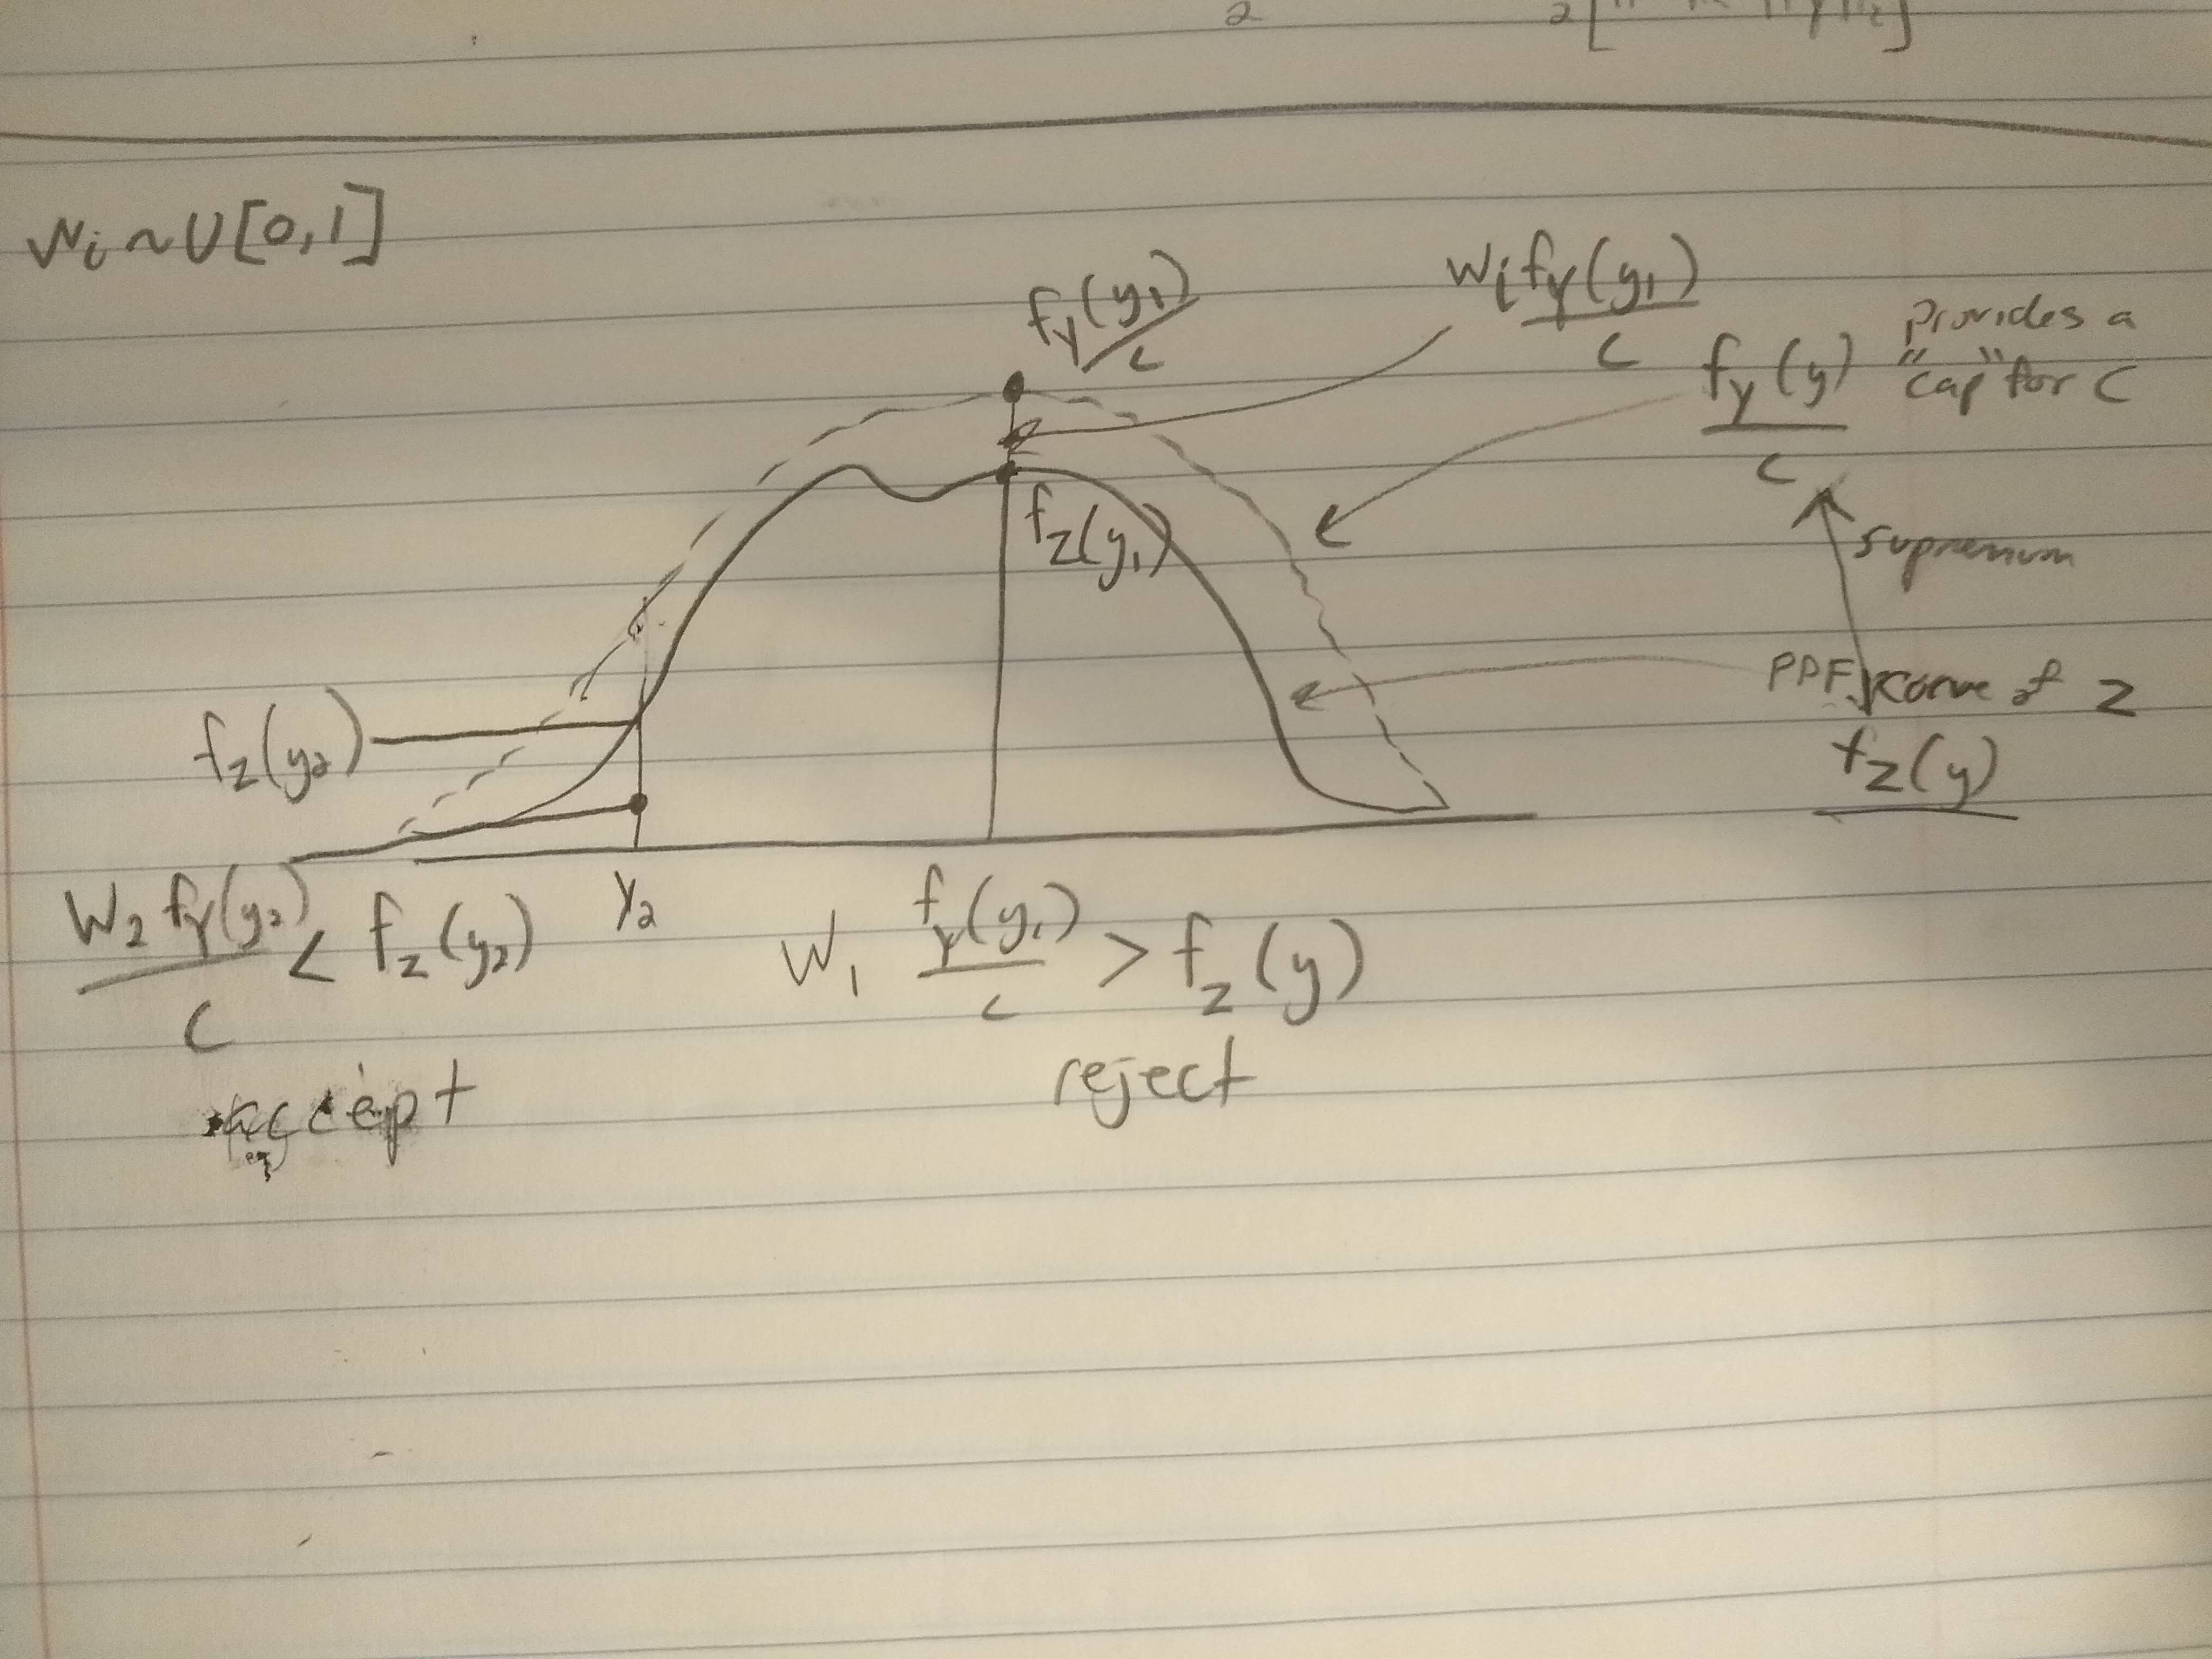
\includegraphics[width=.9\linewidth]{./resources/acceptreject.jpg}
\end{center}


\subsubsection{Proof}
\label{sec:org129ebc9}

How do we know whether the accepted samples are sufficient for a random sample?

\begin{equation}
\begin{split}
\lim_{\Delta \to 0} & \frac{P(Y \in [y, y + \Delta] | \ \text{Y accepted to be Z})}{\Delta} = f_Z (y)\\
\lim_{\Delta \to 0} & \frac{P(Y \in [y, y + \Delta] \cap \ \text{Y accepted to be Z})}{\Delta \cdot P(\text{Y accepted to be Z})}\\
\lim_{\Delta \to 0} & \frac{f_Y(y) \times P(W \leq c f_Z(y)/ f_Y(y))}{\Delta \cdot c} & \ \text{Using definition for P(Y is Z)}\\
\lim_{\Delta \to 0} & \frac{f_Y(y) \times c f_Z(y)/ f_Y(y)}{c} = f_Z (y)
\end{split}
\end{equation}

\begin{equation}
\begin{split}
P(\text{Y accepted to be Z}) = & \lim_{n \to \infty} \sum_{i = 1}^{n} P (w \leq \frac{c f_Z (y_i)}{f_Y (y_i)}) f_Y (y_i) \cdot \Delta\\
= & \lim_{n \to \infty} \sum_{i = 1}^{n} P (\text{accept } y_i | y_i) \cdot P(y_i)\\
= & \int_\Omega \frac{c f_Z (y_i)}{f_Y (y_i)} \cdot f_Y (y_i) dy\\
= & c \int_\Omega f_Z (y) dy\\
= & c \cdot 1 = c
\end{split}
\end{equation}

\(\Omega\): Support of Y and Z

\begin{itemize}
\item You \textbf{must} know the PDF function \(f_Y, \ f_Z\) explicitly
\item Generating \$Y\textsubscript{1}, Y\textsubscript{2},\ldots{}\$ with PDF \(f_Y\) may be done using the inverse
transformation method.
\end{itemize}

\subsubsection{Application}
\label{sec:org9346ffd}

Generate a Sequence of 1000 random numbers.

$$
f_Z (z) = 20z (1 - z)^3, \ 0 < z < 1, \ z \sim Beta(\alpha = 2, \beta = 4)
$$

\(f_Y \sim U[0,1]\)

\begin{enumerate}
\item The candidate distribution \(f_Y(y) = 1, \ 0 < y < 1\)
\item What is the value of C?

$$
   \frac{1}{c} = sup \ \frac{f_Z(y)}{f_Y(y)}
   $$

\(Q = \frac{f_Z(y)}{f_Y(y)} = \frac{20z(1 - z)^3}{1}\).  Need to find max of Q

\begin{subequations}
\label{first:main}
\begin{align}
\frac{dQ}{dz} = & 20 z(1 - z)^3 - 60z(1 - z)^2\\
= & (1 - z)^2 (20 (1 - z) - 60z)\\
= & (1 - z)^2 (20 - 80z) = 0\\
z = & 1, \frac{1}{4}
\end{align}
\end{subequations}

Since \(\frac{1}{4}\) is the smallest,

$$
    \frac{20 (0.25)(1 - 0.25)^3}{1} = \frac{135}{64} \to \frac{1}{c} \to c = \frac{64}{135}
    $$

\item How many random samples are required?

Let N be the number of iterations required.

\(E(N) = \frac{1000}{c} = \frac{1000 \cdot 135}{64} = \frac{135000}{64}\)

\(N = 1.1 \cdot E(N) = 2321\) random samples

\item How to simulate

\begin{enumerate}
\item Sim N random samples from \(U[0,1]\) Y
\item Sim N random samples from \(U[0,1]\) W
\item Make decision. if \(W_i < \frac{c f_Z(y)}{f_Y(y)}\) then reject
\end{enumerate}
\end{enumerate}
\subsubsection{Normal Distribution}
\label{sec:org063dc82}

\(f_Z (z) = \frac{1}{\sqrt {2 \pi}} exp(-z^2/2), \ \ - \infty \leq z \leq \infty\)

Want to simulate a Normal Z but we need to find a candidate distribution with
the same support. No other distributions have the same support as the Normal but
many have the support \(0 \leq y < \infty\).

\(|z| < \infty\)

\begin{equation}
\begin{split}
P(|z| \leq z) = & P(-z \leq Z \leq z)\\
= & \Phi (z) - \Phi(-z)\\
= & \Phi (z) - (1 - \Phi (z))\\
= & 2 \Phi (z) - 1
\end{split}
\end{equation}

\(f_{|z|} (z) = \frac{2}{\sqrt{2 \pi}} exp(- z^2/2)\)

\(P(z < 0) = P(z \geq 0) = 0.5\)

We will need to simulate random samples from \(|z|\).

\begin{enumerate}
\item What is the candidate distr. for Y?

$$
   Y \sim exp(1), \ \ f_Y(z) = exp(- z), \ 0 \leq z < \infty
   $$

\item What is the value of c?

$$
   Q = \frac{1}{c} = \frac{f_Z(z)}{f_Y(z)} = \frac{\frac{2}{\sqrt{2 \pi}}
   exp(-z^2/2)}{exp(-z)} = \frac{2}{\sqrt{2 \pi}} exp(-z^2/2 + z)
   $$

Maximize Q which means maximize \(-z^2/2 + z\) (z = 1)

\(Q = \frac{2}{\sqrt{2 \pi}} exp(0.5) = \sqrt{\frac{2e}{\pi}} = \frac{1}{6}\)

\(c = \sqrt{\frac{\pi}{2e}}\)

\(Q = \frac{1}{c} = \frac{c f_Z(y)}{f_Y(y)} = sqrt{\frac{\pi}{2e}} \cdot \sqrt{\frac{2}{\pi}} exp(-z^2/2 + z) = exp(-z^2/2 + z - 0.5)\)

\(c \frac{f_Z(y)}{f_Y(y)} = exp(- \frac{y^2}{2} + y - 0.5) = exp(-\frac{1}{2}(y - 1)^2)\)

\item How many random samples?

\(E(N) = \frac{1000}{c} \approx 1316\)

\(N = 1.1 \cdot 1316 = 1448\) random samples

\item Simulate

\begin{enumerate}
\item Simulate R.S \(U[0,1]\) W
\item Simulate \$.S from \(Y \sim exp(1)\)
Inverse transformation method yields \(Y_i = - log(x_i)\)

\begin{equation}
\begin{split}
F_Y(y) = & 1 - e^{-1}\\
F_Y^{-1}(x) = & -log(x_i) OR \ -log(1 - x_i)
\end{split}
\end{equation}

\item If \(W_i \leq exp(-0.5(y - 1)^2)\), accept.
\item Simulate R.S \(V_i \sim U[0,1]\)

\(Z_k = sign(V_i - 0.5) Y_i\)
\end{enumerate}
\end{enumerate}

\subsection{Brownian Motion Time Differencing}
\label{sec:orgba81177}

Sometimes instead of a scalar, we want to generate random functions, \(B\).

\subsubsection{Properties}
\label{sec:orga2693a8}
\begin{itemize}
\item \(B(0) = 0\)
\item \(B(\tau)\) and \(B(t) - B(\tau)\) are indep for all \(0 \leq \tau \leq t\)
\item \(B(t) - B(\tau) \sim N(0, t - \tau)\)
\item \(B(t)\) and \(B(\tau)\) are \uline{not} independent.
\(cov(t, \tau) = min(t, \tau) = \tau\)
\item May be generated at discrete times, \(0 = t_0 < t_1 < ... < t_\alpha = T\)

\(B(0) = 0, B(t_k) = B(t_{k - 1}) + X_k \sqrt{t_k - t_{k - 1}}, k = 1,...,d\)

\(X_1,...,X_d\) are iid.
\end{itemize}

\subsubsection{Linear Interpolation}
\label{sec:org394ef50}

\begin{figure}[htbp]
\centering
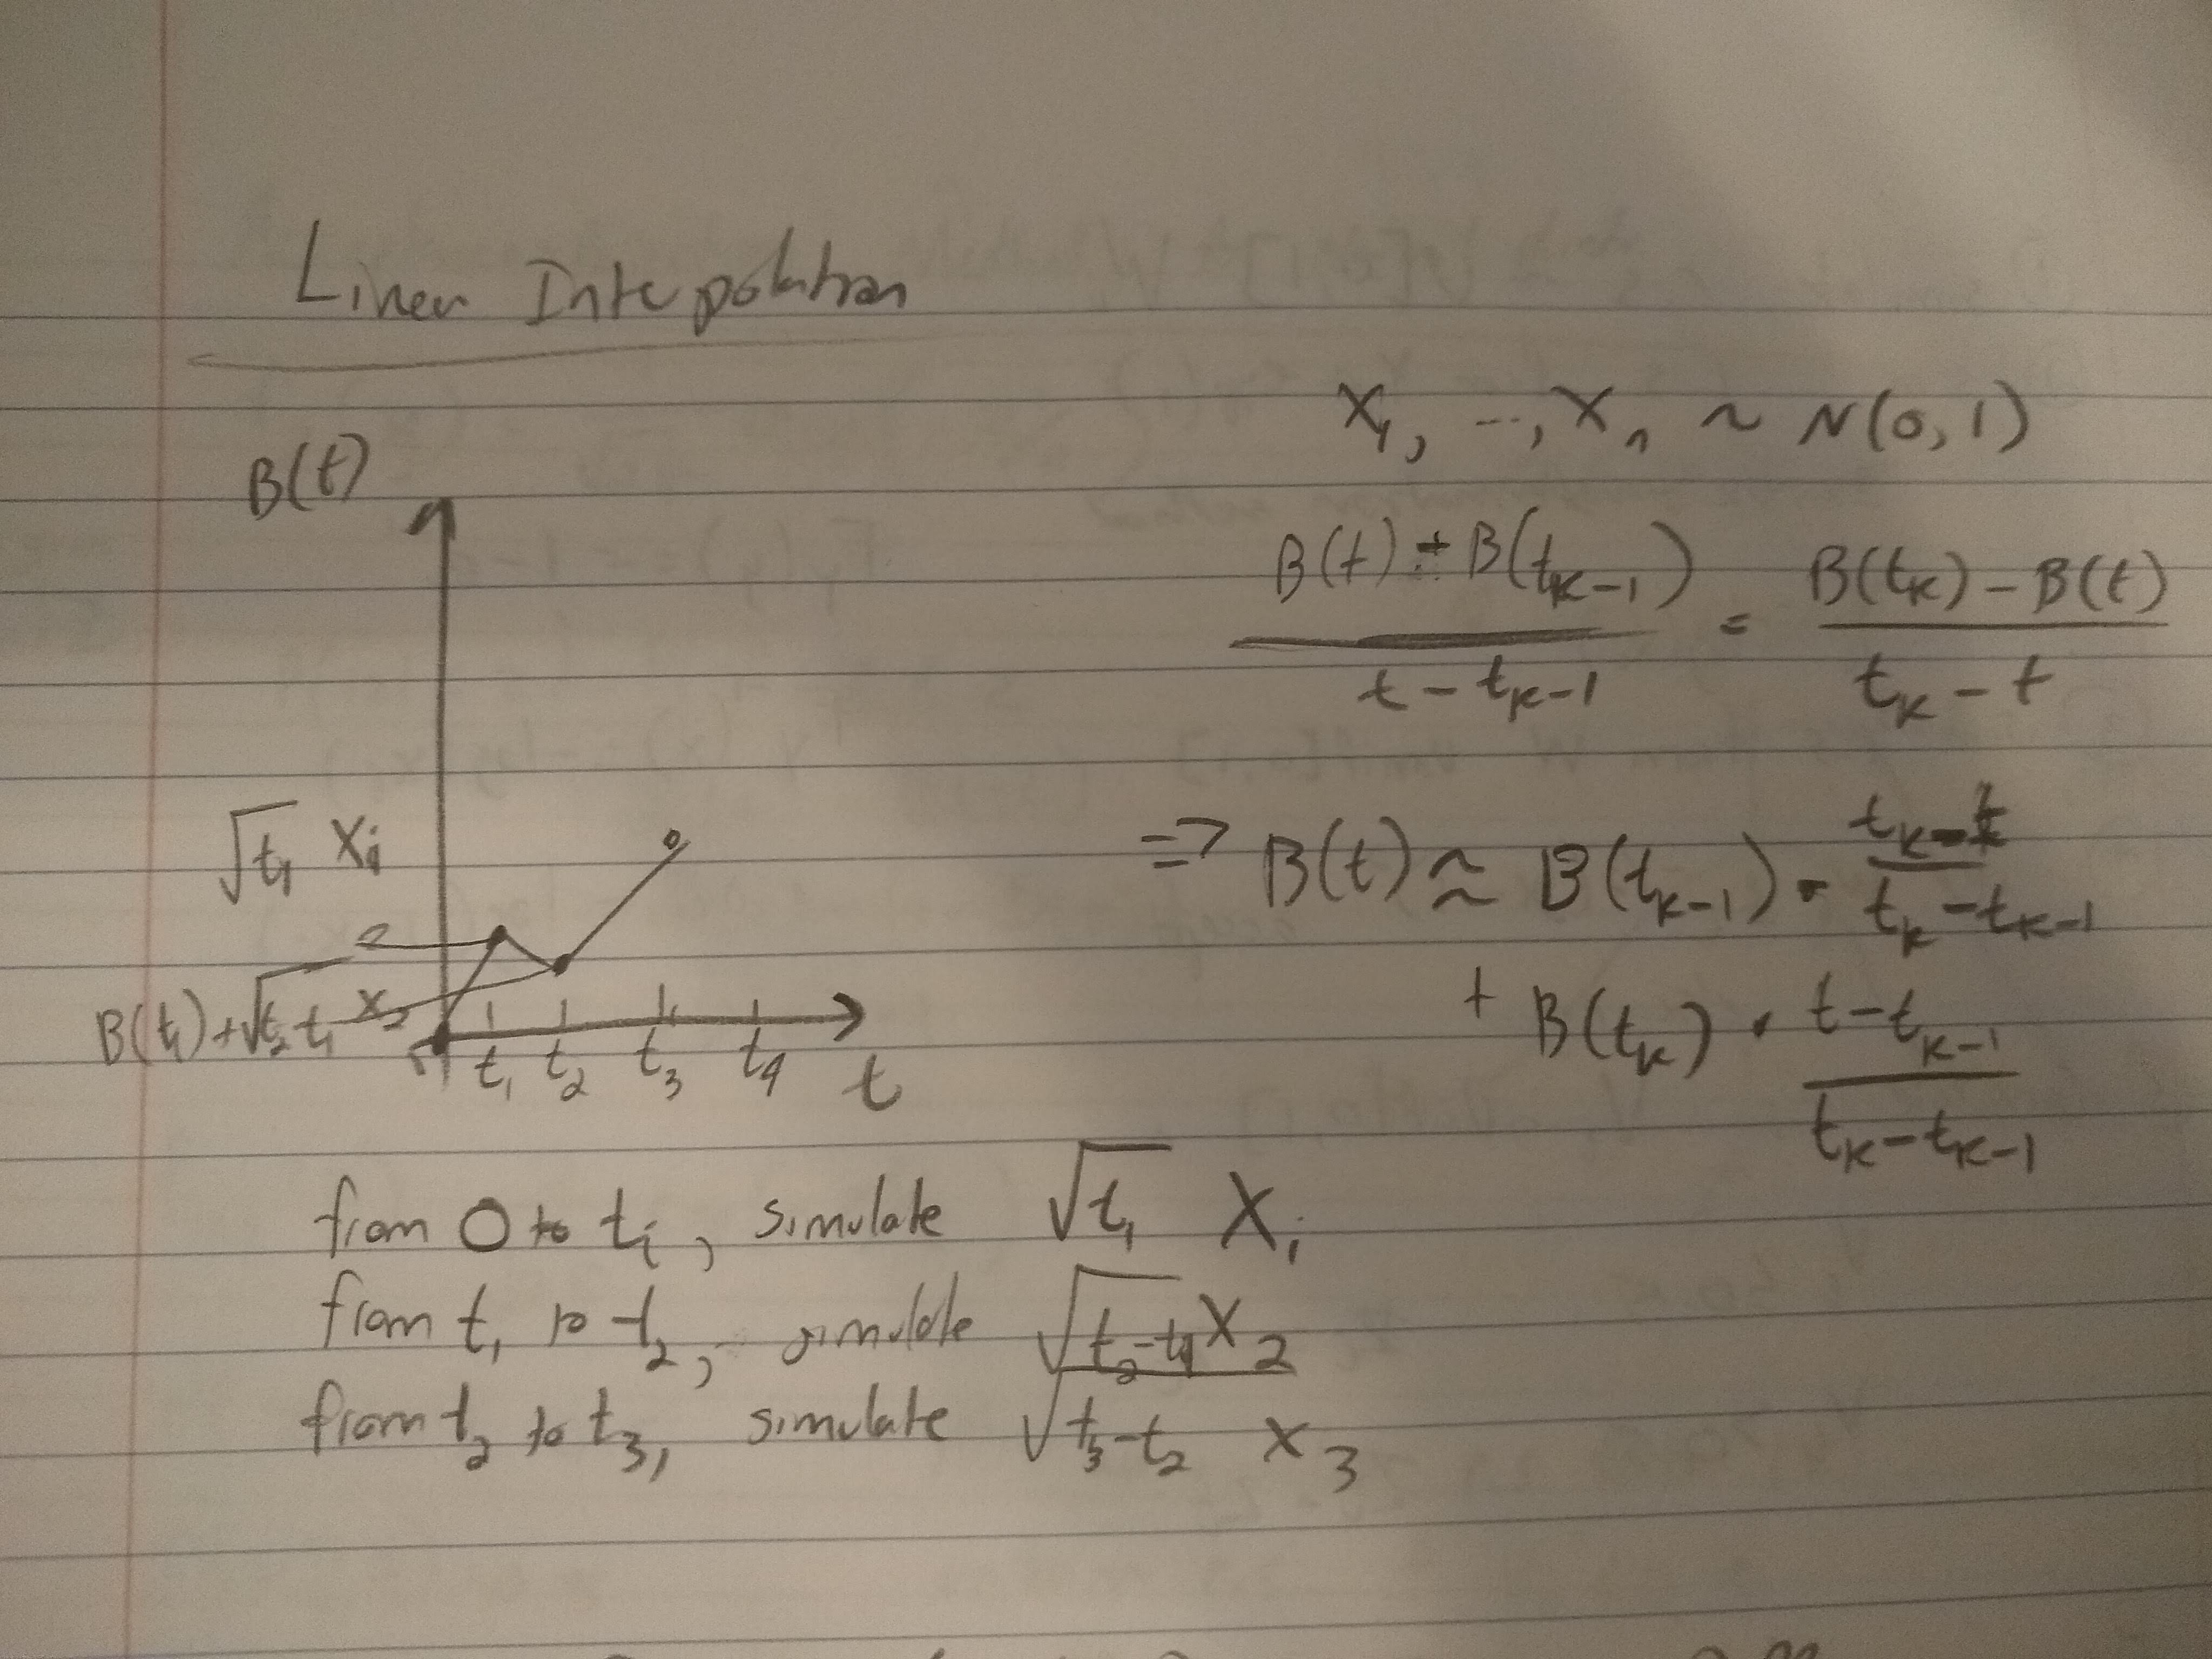
\includegraphics[width=10.6cm,height=7cm\textwidth]{./resources/linear_interpolation.jpg}
\caption{\label{fig:org4ba9163}Linear Interpolation}
\end{figure}

\subsubsection{Generating Brownian Sample Paths}
\label{sec:org78a9e99}

\(d\): number of time nodes

$$
0, \frac{T}{d}, \frac{2T}{d}, ..., \frac{(d - 1)T}{d}, \frac{dT}{d} = T
$$

to generate sample paths of brownian motion.

\begin{enumerate}
\item Generate \(d\) standard normal random numbers \(X_1, ..., X_d\)
\item Brownian motion at time \(\frac{kT}{d}, \ k = 1,2,...,d\)
\end{enumerate}

\_\textsubscript{Relationship} between Brownian Motion and Geometric Brownian Motion\_

They are the same thing.

\emph{Brownian Motion}

$$
S(T) = S(0) exp(rT - T\frac{\sigma^2}{2} + \sigma B(T))
$$

\emph{Geometric Brownian Motion}

$$
S(T) = S(0) exp(T(r - \frac{\sigma^2}{2}) + \sigma B(T))
$$

\section{Types of Options (2020/05/14)}
\label{sec:orgfc90928}
\subsection{Vanilla European Call/Put Option}
\label{sec:org0ddb6b2}
\begin{quote}
Asset path not important for European options
\end{quote}

\textbf{Review}

$$S(t) = S(0) exp(r - \sigma^2/2)t + \sigma B(t) = S(0) exp(r -
    \sigma^2/2)t + \sigma \sqrt{t} X$$

\(\sqrt T X \approx B(t)\)

where \(X \sim N(0,1)\)

\(E(S(t)) = S(0) exp(rt)\)

\begin{equation}
\begin{split}
S(\frac{t}{d}) = & S(0) exp(r - \sigma^2/2) \frac{t}{d} + \sigma \sqrt{\frac{t}{d}} X_1\\
S(\frac{2t}{d}) = & S(0) exp(r - \sigma^2/2) \frac{2t}{d} + \sigma \sqrt{\frac{t}{d}} (X_1 + X_2)\\
S(\frac{3t}{d}) = & S(0) exp(r - \sigma^2/2) \frac{3t}{d} + \sigma \sqrt{\frac{t}{d}} (X_1 + X_2 + x_3)\\
...\\
S(t) = & S(0) exp(r - \sigma^2/2)t + \sigma B(t) = S(0) exp(r - \sigma^2/2)t + \sigma \sqrt{t} X
\end{split}
\end{equation}


More generically,

$$
S(\frac{kt}{d}) = & S(0) exp(r - \sigma^2/2) \frac{kt}{d} + \sigma
\sqrt{\frac{t}{d}} \sum_{1}^{k} X_i\\
$$

where \(\sum_{i}^{k} X_i \sim N(0, \frac{kt}{d})\)

\(d\): Number of increments. It can be years, days, hours, etc. In previous
discussions, d was \emph{years}. In this case, it is \emph{days}.

\textbf{Simulation Steps}
\begin{enumerate}
\item Simulate independent Std. Norm R.V.s \(n \times d\)
\item Generate Brownian Motion Path for each sample
\(\sqrt{\frac{t}{d}} \cdot cumsum(x)\)
\item Generate Geometric Brownian Motion using formula above (asset price path)
payoff = \(max(K - S(t), 0)\)
discounted payoff = \(max(K - S(t), 0) exp(-rt)\)
\end{enumerate}

\subsection{Asian Call/Put Options}
\label{sec:org499ccc3}

Uses the average price of the asset from purchase to maturity instead of the
asset price at maturity.

European Option = Arithmetic or Geometric Asian Option where d = 1.

\(\bar S_{geo} \leq \bar S_{ari}\)

\subsubsection{Arithmetic Mean}
\label{sec:orgd1c9003}

call payoff = \(max(\frac{1}{d} \sum_{j = 1}^{d} S(\frac{jT}{d}) - K, 0)\)

put payoff = \(max(K - \frac{1}{d} \sum_{j = 1}^{d} S(\frac{jT}{d}), 0)\)

European options will be a higher payout because of higher volatility.

\subsubsection{Geometric Mean}
\label{sec:org859f16b}

\(\sqrt{ab}\)

$$
\bar S_{geo} = [ \Pi_1^d S(\frac{jT}{d})]^{1/d}
$$

\begin{equation}
\begin{split}
S(\frac{T}{d}) = & S(0) exp((r - \sigma^2/2)\frac{T}{d} + \sigma \sqrt{\frac{T}{d}} X_1)\\
S(\frac{2T}{d}) = & S(0) exp((r - \sigma^2/2)\frac{2T}{d} + \sigma \sqrt{\frac{T}{d}} (X_1 + X_2))\\
...\\
S(T) = & S(0) exp((r - \sigma^2/2)T + \sigma \sqrt{\frac{T}{d}} \sum_{1}^{d} X_i)\\
\end{split}
\end{equation}


\begin{equation}
\begin{split}
[ \Pi_1^d S(\frac{jT}{d})]^{1/d} = & [S(0) exp(d(r - \sigma^2/2) \frac{(1 + 2 +
... + d) T}{d} + \sigma \sqrt{\frac{T}{d}} [X_1 + (d - 1) X_2 + (d - 2) X_3 +
... + X_d])]^{1/d}\\
= & S(0) [exp((r - \sigma^2/2)\frac{d(d + 1)}{d} \cdot \frac{T}{d} + \sigma \sqrt{\frac{T}{d}} W)]
\end{split}
\end{equation}

\(W = d X_1 + (d - 1) X_2 + ... + x_0 d \sim N(0, \frac{d(d + 1)(d + 2)}{6})\)

\(V(W) = d^2 + (d - 1)^2 + ... + 1^2 = \frac{d(d + 1)(d + 2)}{6}\)

We replace W with \(\sqrt{\frac{d(d + 1)(d + 2)}{6}} X\)

\(T = (\frac{d + 1}{2d})T = (\frac{1}{2} + \frac{1}{d})T \leq T\)

\(\bar \sigma^2 = \frac{\sigma^2 (2 + \frac{1}{d})}{3} = (\frac{2}{3} + \frac{1}{3d}) \sigma^2 \leq \sigma^2\)


\(r = r + (\bar \sigma^2 - \sigma^2)/2 \leq r\)

\subsection{Barrier Options}
\label{sec:orgd4a28aa}

There may be a barrier price, b, which one must cross to trigger the option (one
way or another).

\subsubsection{Knock-in Barrier Option}
\label{sec:org029df39}

\begin{quote}
Knock-out is the opposite of Knock-in. I.e. option no longer valid if the
barrier is crossed.
\end{quote}
\begin{enumerate}
\item Up-and-in
\label{sec:orge9a2ded}
If barrier is met during the time to maturity, the option is activated.

\begin{figure}[htbp]
\centering
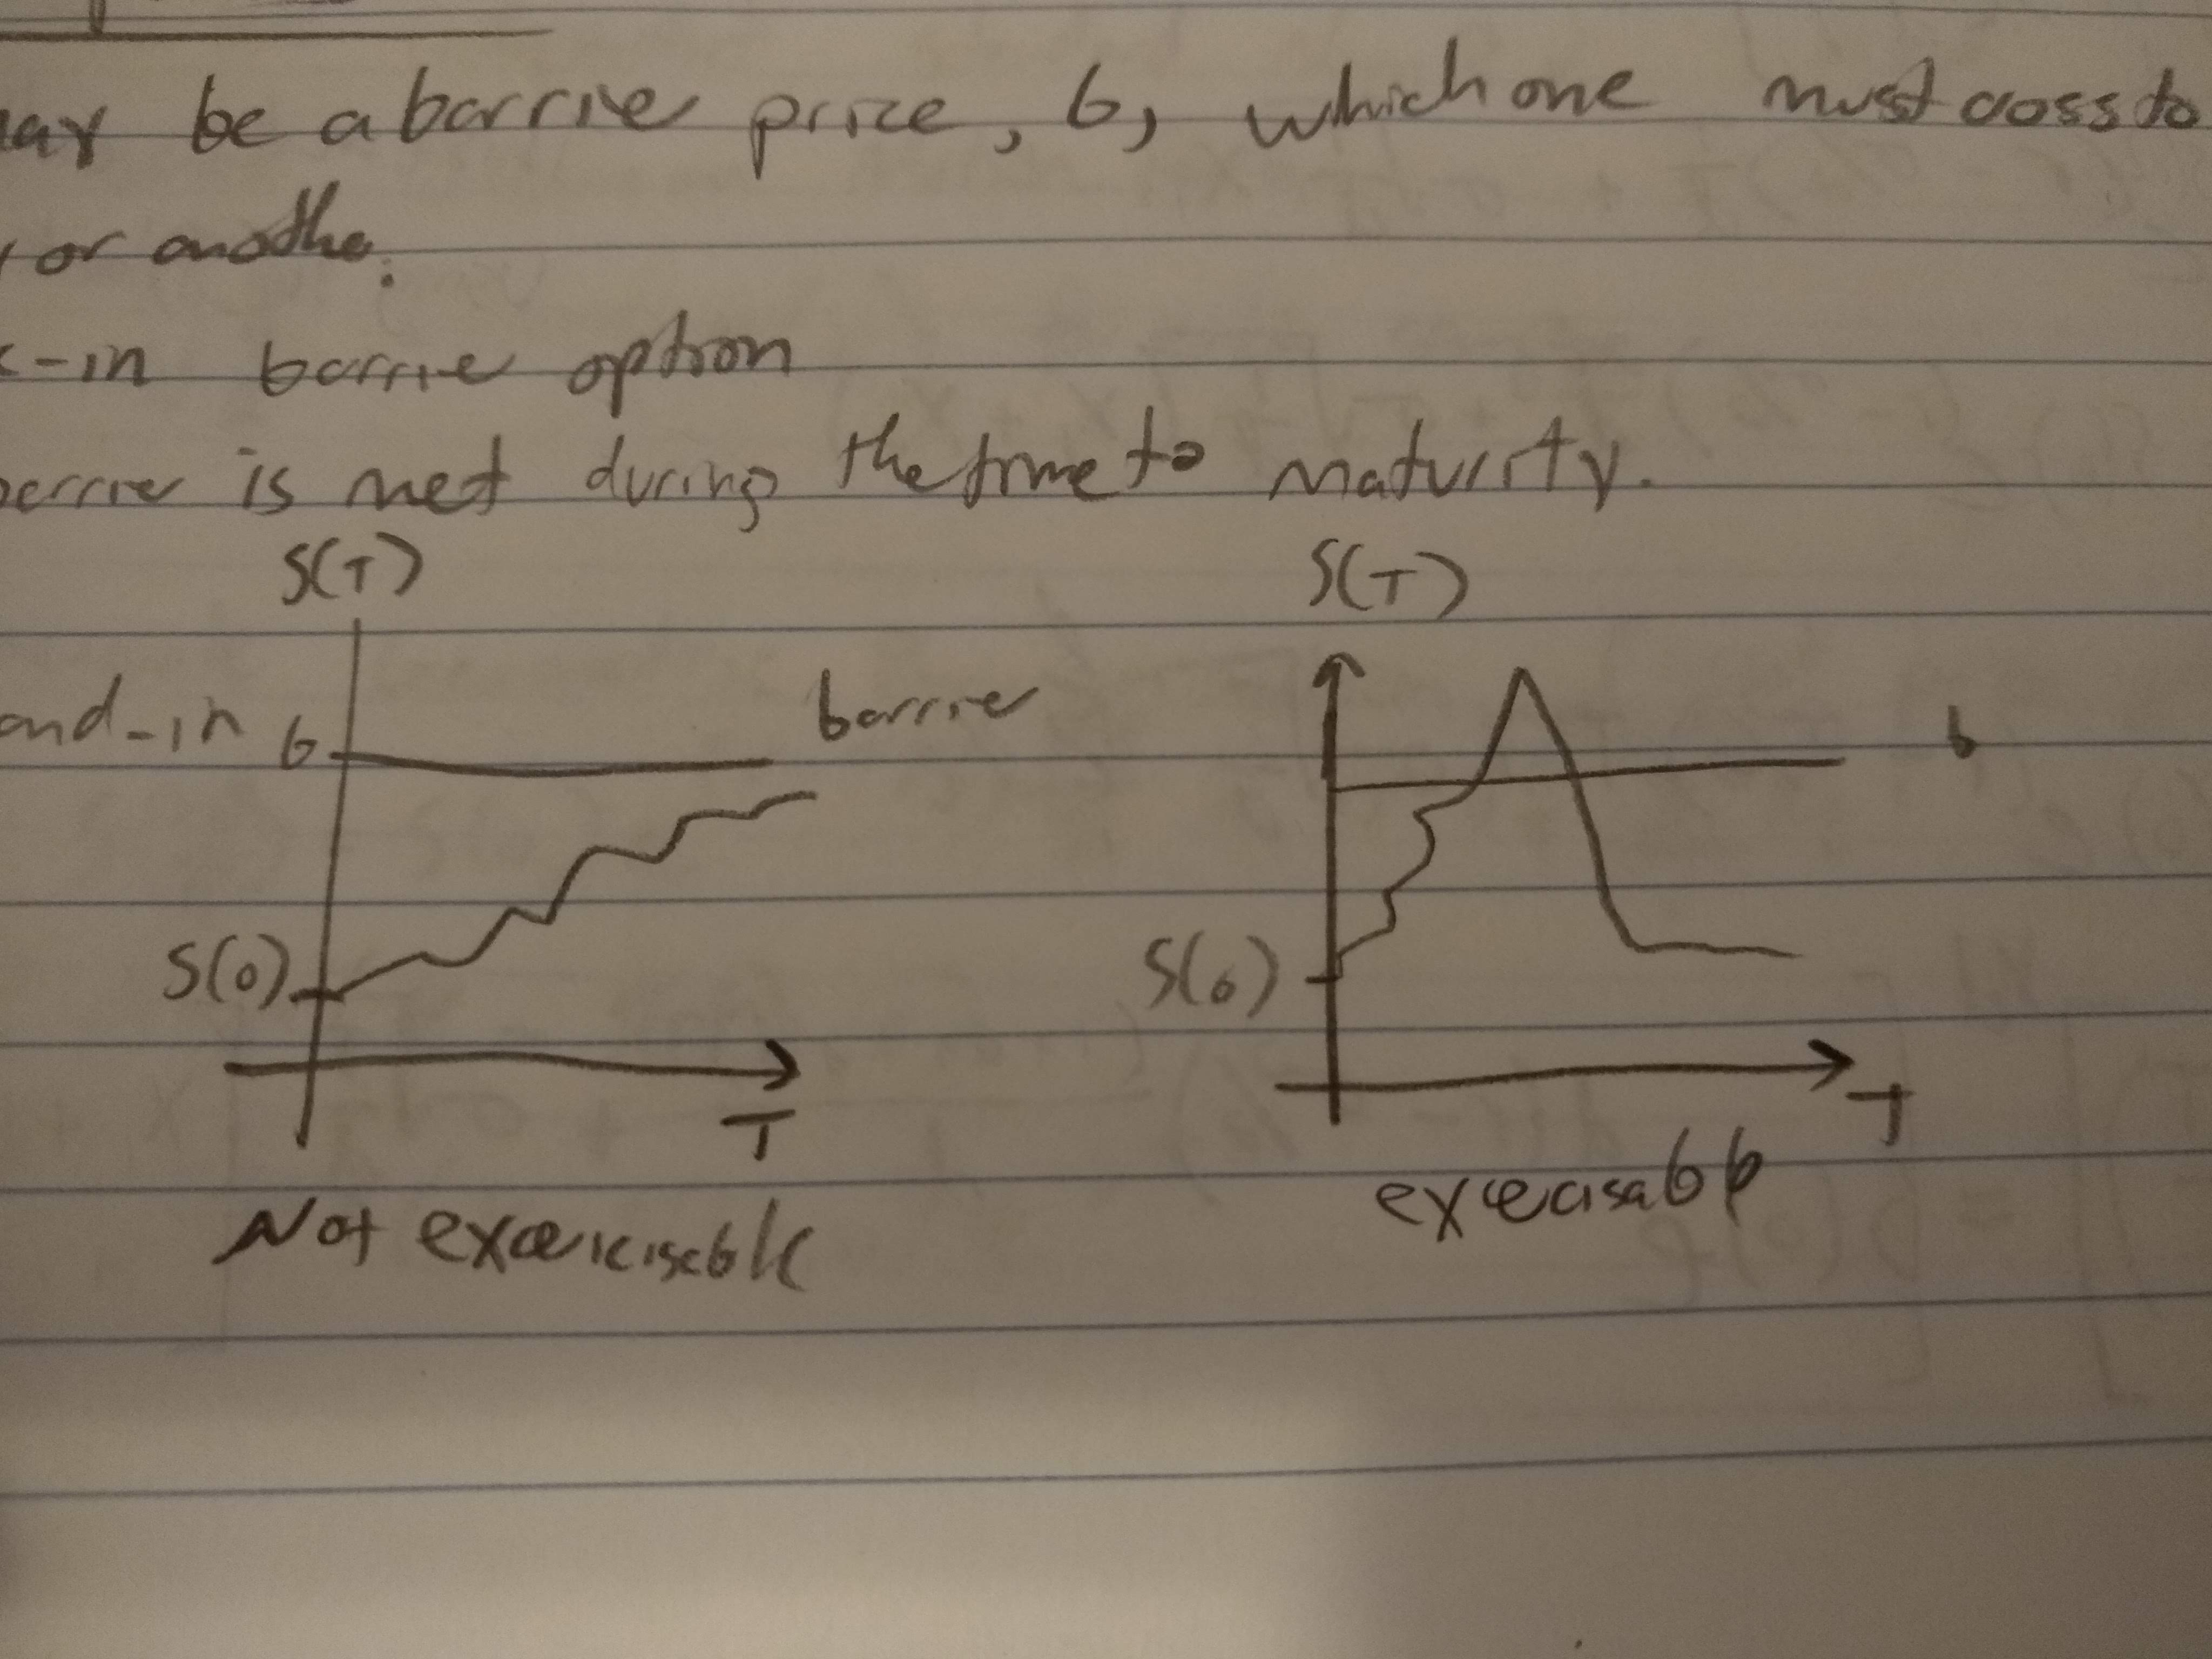
\includegraphics[width=.9\linewidth]{./resources/barrier_options.jpg}
\caption{\label{fig:orga6d9573}Barrier Options: Up and In}
\end{figure}

\item Down-and-out
\label{sec:org5b93fc2}

\begin{figure}[htbp]
\centering
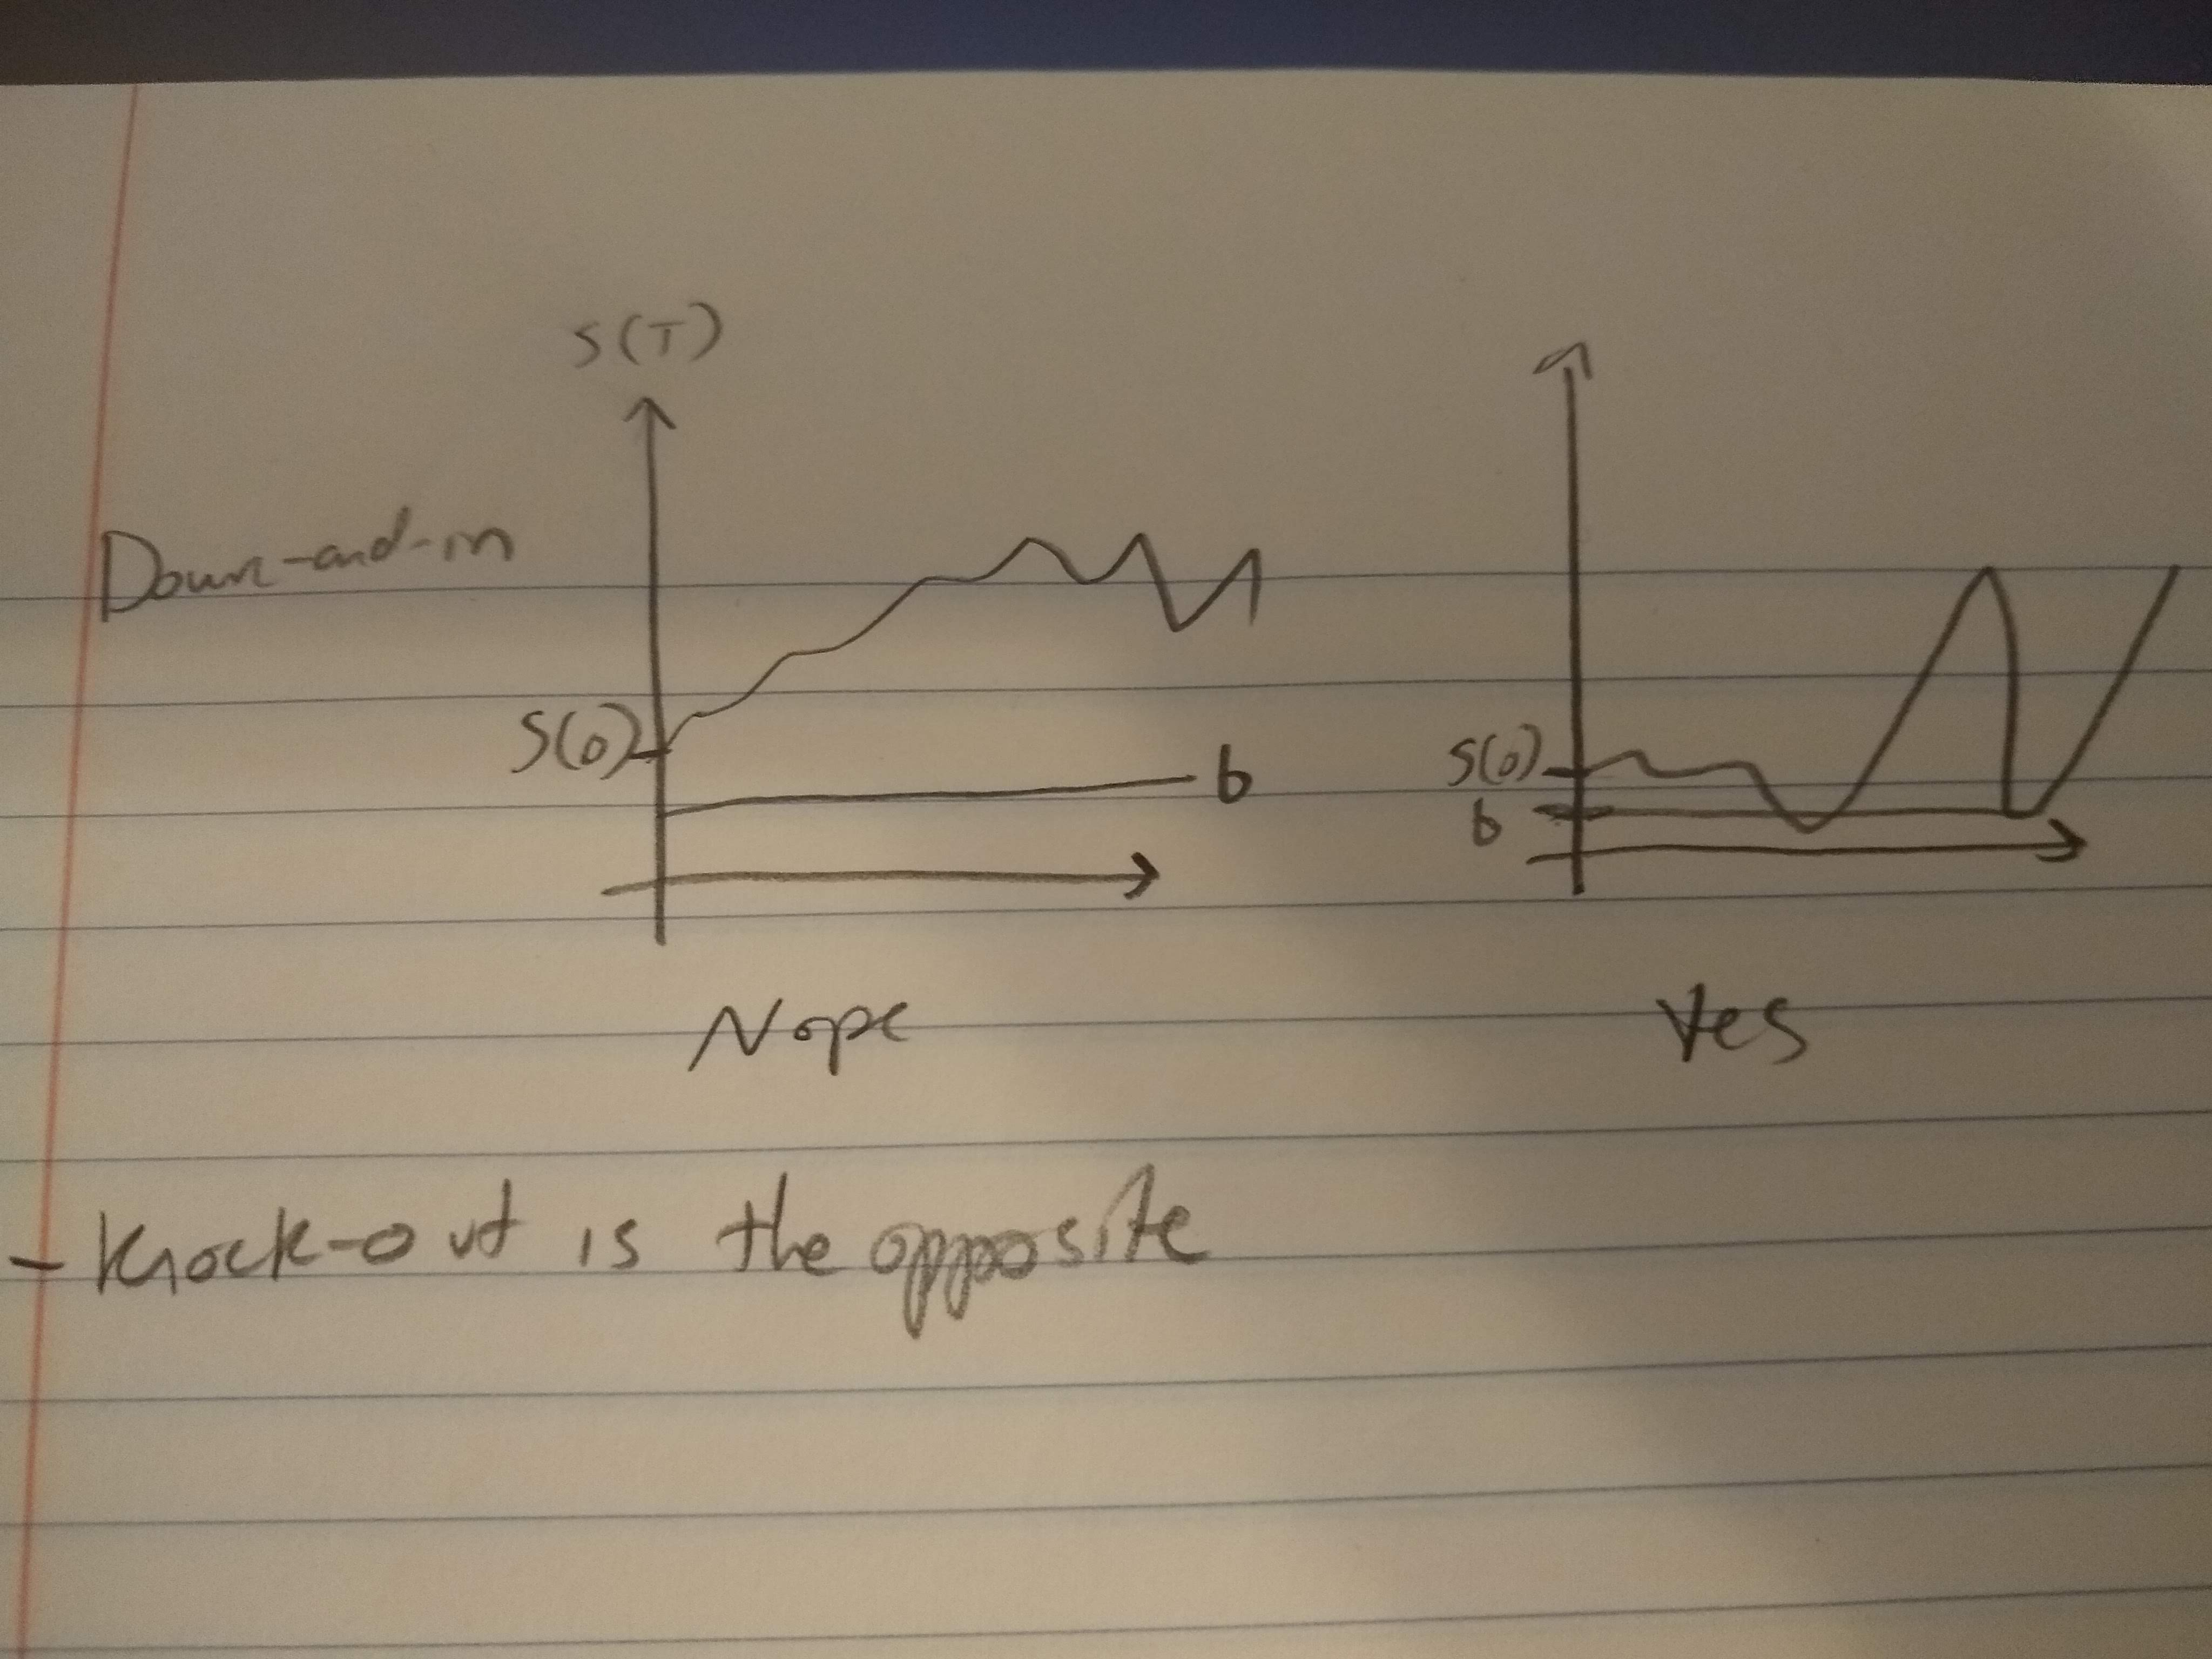
\includegraphics[width=.9\linewidth]{./resources/barrier_downandout.jpg}
\caption{\label{fig:orgf01a383}Barrier Options: Down and Out}
\end{figure}
\end{enumerate}


\subsection{Lookback Options}
\label{sec:org583c1b3}

Minimum or maximum value of the asset price before expiry acts as a strike
price.

Call Payoff

$$
S(T) - \min_{j = 1,...,d} S(jT/d) \ \text{or} \ S(T) - \min_{0 < t \leq T} S(t)
$$


Put Payoff

$$
\max_{j = 1,...,d} S(jT/d) - S(T) \ \text{or} \ \max_{0 < t \leq T} S(t) - S(T)
$$
\section{Control-Variate Method for Efficiency (2020/05/21)}
\label{sec:org55d48b9}

Suppose we want to estimate estimate \(\mu = E(Y)\).

Possible estimators
\begin{itemize}
\item \(\bar Y\)
\item \(Y_1\)
\item \(Y_1 + \frac{Y_2 + Y_3}{2}\)
\end{itemize}

\(\hat \mu\) is a point estimator of \(\mu\).

How do we evaluate a point estimator? MSE

\begin{equation}
\begin{split}
MSE = & E((\hat \mu - \mu)^2)\\
= & Var(\hat \mu) + Bias^2(\hat \mu)
\end{split}
\end{equation}

Let Y be a R.V. whose \(\mu\) you want to estimate.
Let X be a R.V. whose \(\mu_x\) you already know.

\uline{Example}

A student takes two tests. We would like to estimate the score of the second
test. We know the distribution and score of the first test. The second test is
\emph{correlated} with the score of the first. For example, if they do well on the
first exam, it is likely that they will do well on the second exam.

\(X \sim N(85, 5^2), \ W \sim N(0, 3^2)\)

\(Y = X + W\)

\(X\) in this case is the \textbf{variate}. The \textbf{Control Variate} means Control \(X\).

Let \((X_i, Y_i), \ i = 1,...,n\) be iid draws of \((X, Y)\) which are not
independent of each other.

$$
\hat Y = \bar Y + \beta(\mu_X - \bar X)\\ E(\hat Y) = \mu
$$

Without X, \(\bar Y\) is an unbiased estimator for \(\mu\).

\(V(\bar Y) = \frac{\sigma^2}{n}\)

\(V(\hat Y) = V(\bar Y) + \beta(\mu_X - \bar X)\)

We would like to choose \(\beta\) such that \(Var(\hat Y)\) is minimized.


\begin{equation}
\begin{split}
\hat Y = & \frac{Y_1 + ... + Y_n}{n} + \frac{\beta (\mu_X - (x_1 + ... + x_n))}{n}\\
= & \frac{1}{n} \sum_{1}^{n} Y_i + \beta (\mu_X - X_i)
\end{split}
\end{equation}

Adjust \(\mu_X - X_i\) to be closer to the mean. This reduces variance of the
point estimator.


\begin{equation}
\begin{split}
V(\hat Y) = & V(\bar Y + \beta (\mu_X - \bar X))\\
= & V(\bar Y) + V(\beta (\mu_X + \bar X)) + 2 cov (\hat Y, \beta (\mu_X - \bar X))\\
= & \frac{\sigma^2}{n} + \beta^2 \frac{\sigma_X^2}{n} - 2 \beta cov(\bar Y, \bar X - \mu_X)
\end{split}
\end{equation}


\begin{equation}
\begin{split}
cov(\bar Y, \bar X) = & cov(\frac{Y_1 + ... + Y_n}{n}, \frac{X_1 + ... + X_n}{n})\\
= & \frac{n}{n^2} cov (X, Y)\\
= & \frac{cov(X, Y)}{n} = \frac{corr(X, Y) \sigma_x \sigma_y}{n}
\end{split}
\end{equation}

$$
\frac{\partial V(\hat Y)}{\partial \beta} = \frac{2 \beta \sigma_X^2}{n} -
\frac{2 corr(X, Y) \sigma_x \sigma_Y}{n} = 0
$$

\(\beta = \frac{corr(X, Y) \sigma_X \sigma_Y}{\sigma_X} =
\frac{cov(X,Y)}{\sigma_X^2} = \frac{\sigma_{xy}^2}{\sigma_x^2}\)


\begin{equation}
\begin{split}
V(\hat Y) = & \frac{\sigma_Y^2}{n} + (\frac{\sigma_{xy}^2}{\sigma_X}^2)^2 \frac{\sigma_X^2}{n} - \frac{2 \sigma_{xy}^2}{\sigma_X^2} - \frac{\sigma_{xy}^2}{n}\\
= & \frac{\sigma_Y^2}{n} + \frac{\sigma_{xy}^4}{\sigma_X}^4 \cdot \frac{\sigma_X^2}{n} - \frac{2 \sigma_{xy}^4}{n \sigma_X^2}\\
= & \frac{\sigma_Y^2}{n} + \frac{\sigma_{xy}^4}{n \sigma_X^2}\\
= & \frac{\sigma_Y^2}{n}[1 - \frac{\sigma_{xy}^4}{\sigma_X^2 \sigma_Y^2}] = \frac{\sigma_Y^2}{n}[1 - corr(X,Y)]
\end{split}
\end{equation}

The larger the correlation, the \textbf{better}.


\(V(\bar Y) = \frac{\sigma_Y^2}{n}\)

$$RMSE (\hat Y) = \sqrt{Var(\hat Y)} = \frac{\sigma_Y}{\sqrt n} [1 - corr^2(X, Y)]^{1/2}$$

Choosing the Control Variate, X, to mark Corr(X, Y) as close to \(\pm 1\) as
possible.

\begin{equation}
\begin{split}
\hat Y = & \bar Y + \hat \beta (\mu_X - \bar X) = \bar Y + \frac{(\mu_X - \bar X) \sum_{1}^{n}(X_i - \bar X)(Y_i - \bar Y)}{\sum_{1}^{n} (X_i \bar X)^2}\\
= & \sum_{1}^{n} W_i Y_i \ \text{where} \ w_i = \frac{1}{n} + \frac{(\mu_X - \bar X)(X_i - \bar X)}{\sum_{1}^{n} (X_i - \bar X)^2}
\end{split}
\end{equation}

If \(X_i < \bar X\) and \(\mu_X > \bar X\), then opposite side of \(\bar X\) has a
negative weight. Otherwise, its positive.


\textbf{Remarks}
\begin{itemize}
\item X,Y must be highly correlated
\item All pairs of X,Y must be independent
\item Reduces MSE but doesn't necessarily lead to a more accurate estimator.
\end{itemize}
\end{document}
